\ifpdf
    \graphicspath{{Chapter6/Figs/Raster/}{Chapter6/Figs/PDF/}{Chapter6/Figs/}}
\else
    \graphicspath{{Chapter6/Figs/Vector/}{Chapter6/Figs/}}
\fi


\chapter[State of the Art White Supremacy: On Disembodiment in the Machine Learning Pipeline]{State of the Art White Supremacy: On Disembodiment in the Machine Learning Pipeline\footnotemark{}}\label{chap:disembodied}
\chaptermark{State of the Art White Supremacy}
\footnotetext{This chapter contains elements from a collaboration with Smarika Lulz, Joachim Bingel, and Isabelle Augenstein. The associated paper is currently under review in the journal Computational Linguistics. The title is taken from a conversation between Abeba Birhane, Chris Dancy and me, where Chris offered the term State-of-the-Art White Supremacy.}

\begin{citequote}{\citet[p.110-111]{Lorde:1984}}
What does it mean when the tools of a racist patriarchy are used to examine the fruits of that same patriarchy?  It means that only the most narrow parameters of change are possible and allowable.
\end{citequote}

In each of the previous chapters we have identified different areas of concern for the use of models and data. From the constraints of document transformation in \autoref{chap:liwc} to the influence of multiple data sources and prediction tasks in \autoref{chap:mtl}. In this chapter, I theorise over the core sources of these issues: the context within which models and exist, the models and the data.
To describe these issues, I invoke the metaphor of the body in three different ways: first, pertaining to the physical material \textit{human body} that we each possess; second, to signify a collection of observations and data points \textit{created by humans}; third, to refer subjective embodiments, that is how \textit{social and cultural meaning} is embedded in the human experience and derivatives of it, i.e. data created by humans.
Through a consideration of both data generation processes and the modelling stages of the machine learning pipeline, I then apply my theory to the models that I have described in this dissertation in addition to providing a critique of these technologies. 
Finally, I discuss the implications of current practices in machine learning and argue that for machine learning for social prediction tasks to achieve their goals, we must radically reconsider current approaches to better align with the stated aims.

\section{Disembodied Machine Learning}
Machine learning is a practice that is concerned with making decisions based on machine-discernible patterns in observed data. Often, the data upon which machine learning methods are optimised, and later applied to, are `extracted' from the context within which they are created. Through this process of separation of context and datum, an notion of `objectivity' is imposed upon the data and the subsequent operations on the data and their results. Through the repeated separation of datum from context bodies of data, or datasets, are created. These amalgamated bodies of data exist only by virtue of their strict separation from the material bodies that they derive from are then used to optimise machine learning methods. Machine learning method come in two different forms: Supervised learning methods which seek to learn to distinguish between set of bodies of data, and unsupervised models which seek to identify discernible limbs of data within a single body of data. For both supervised and unsupervised models both the underlying data and the model applied to them have strong influences as to what bodies are discovered and what may be discovered within them. As \citet{Benjamin:2019} writes technology operates within social structure `codes [that] operate within powerful systems of meaning that render some things visible, others invisible, and creates a vast array of distortions and dangers'.\vspace{5mm}

In the advent of machine learning, these models were hailed as objective, unimpeded by subjective human biases, and by extension social marginalisation \citep{oneil:2017}. However, an increasing amount of research suggests that social biases are common in machine learning models \citep{Shah:2020,Buolamwini:2018,Agarwal:2018}, and that biases in the underlying data may be exacerbated by the machine learning models \citep{Zhao:2017,Jia:2020}. As a result of this growing awareness, a number of research directions seek to identify \citep{Shah:2020,Bender-Friedman:2018,Mitchell:2019,Buolamwini:2018}, reduce or remove social biases \citep{Zhao:2017,Agarwal:2018,Romanov:2019,Jia:2020} from machine learning models to prevent further marginalisation. Such work assumes that social biases operate within a positivist logic in which the removal social bias is cast as an optimisation problem, i.e. that there is a finite and quantifiable source of bias that can be disentangled, isolated, and mathematically reduced out of the body of data or mathematical model from which the designer of both models and data are removed.

Here, I provide a challenge to such a positivist logic, drawing on work from feminist Science and Technology Studies and examples from Natural Language Processing I argue that bias and subjectivity in machine learning pipelines are inescapable and can therefore not be simply be reduced or removed, for which reason I hold that an ongoing recognition and reflection on our own positions and the imaginary of objectivity found in subjective realities reflect political choices throughout the machine learning pipeline. Through a contextualisation of bias in these terms, I aim to shift the surrounding discourse away from bias an its elimination to subjective positionality and its implications on the machine learning pipeline from data generation to optimised model.

\subsection{Embodiment in the Machine Learning Pipeline}
Through Haraway's \citeyearpar{Haraway:1988} critique of objectivity (see \cref{chap:socialscience} it is possible to understand subjectivity, or bias in machine learning in a way that recognises its potential to create social marginalisation without casting the problem in a positivist, optimisational logic. I argue that the disembodied or objective position exists within the machine learning pipeline at multiple junctions:
\begin{enumerate}
  \item{In the data which is often removed from context and potentially adjudicated by externalised others,}
  \item{in the person designing the experiment and pipeline, and}
  \item{in the model optimised on the disembodied data stemming from embodied data subjects.}
\end{enumerate}
First, as data collection processes require decisions to be made to delineate individual pieces of datum that are relevant to the task from those that are deemed irrelevant, it is often necessary to also create a separation between the person who created the datum and the datum in and of itself. Thus, a datum is removed from the context of its creator. Further, datum is often disassociated with the time and the social and political contexts within which it is created. In the case of supervised machine learning, the datum is then provided to a number of annotators, who frequently are neither the creator of the datum nor necessarily situated with contexts of the creator or the datum. These annotators then determine which limb of data, within the larger body of data, the datum belongs to given a set of criteria for such judgement.
Second, as the designer of the model themselves are frequently removed from the contexts within which the body of data are created, they determine how the data are to be represented through a choice of features, setting limits on vocabularies (see \autoref{chap:intro}), transforming the input (as seen in \autoref{chap:liwc}), and the choice of models with their requirements of representing data.
Third, as machine learning models step through disembodied data and embody it within itself, the model itself manipulates the representations of data to identify discernible boundaries between the limbs of data. In this process, the models further disembody the data from the data itself, operating within an assumption that datum consist of the sum of its parts.

In each of these situations lay value judgements on which perspectives of the data are relevant and which are irrelevant. I observe here a peculiarity of machine learning, as data which is disembodied from its creator then becomes the body of knowledge upon which the machine learning model draws on, implicitly transforming all positions that exist outside of the model's internal body then becomes disembodied from the model. This transformation from disembodied to embodied then can serve as an explanation for calls for `more' and `more diverse' data \citep{Holstein:2019}.
It is worth noting here that the model-embodiment is tacitly acknowledged in the research fields of domain adaptation \citep{Daume:2007} and transfer learning. Through these fields' acknowledgement that to the knowledge held in machine learning models are limited to the domains that are present in the datasets the models are optimised on and that even small perturbations in the input to the model may drastically degrade its performance~\citep{Szegedy:2014,Daume:2007}. These acknowledgements of embodiment exist in a self-contradictory tension with the position of objectivity within which these transfer-learning and domain adaptation methods operate within.

\subsubsection{The Embodied Designer}

Though often referred to as a `researcher' or `developer', I draw on Herbert \citet{Simon:1969} to construct my understanding of a \textit{designer}. I direct attention not to the profession of the individual or team in the machine learning pipeline but instead to the their action.

\begin{citequote}{\citep[p. 111]{Simon:1969}}
  Everyone designs who devises courses of action aimed at changing existing situations into preferred ones.
\end{citequote}

Following \citet{Simon:1969}, the \textit{designer} can then be understood to be anyone in the machine learning pipeline. While this includes annotators in addition to developers and researchers, I direct focus to the last two as as they can direct and supersede the choices of annotators.

Often a lack of diversity in machine learning development teams is cited as a source of socially biased technologies along with corresponding calls for an increase in designers embodying diverse experiences \citep{West:2019}.
Similar to my argument, such calls argue that the embodied designers project an embodiment of self into the technologies they develop through data and modelling choices. This argument, in line with \citet{Haraway:1988} suggests that it is only through the recognition and promoting different embodiments that certain perspectives, understandings, and uses can be achieved.

\subsection{Embodiment in Data}
As \citet{Gitelman:2013} argues, datasets do not exist naturally but must be produced. Considering this production of data through \citet{Haraway:1988}, datasets can be understood as a form of knowledge that is produced through disembodying embodied experiences. Subjectivity can thus stem from a number of sources including the source of the data \citep{Gitelman-Jackson:2013}, the data sampling method \citep{Shah:2020}, and the selection of annotators \citep{Waseem:2016,Derczynski:2016}.

Grounding my discussion in Natural Language Processing, I show how subjectivity manifests itself in machine learning models through a number of meaning-making processes, modelling choices, and data idiosyncrasies. I seek here to highlight the subjective and embodied nature of of data and classifications and that by taking a position of objectivity, we cannot do justice to the needs and wants of individuals or communities.

\subsubsection{Natural Language Processing Tasks}

A range of, if not all, Natural Language Processing tasks are highly sensitive to the subjective values encoded in data. While such issues have frequently been studied in the context of high-level tasks, such as machine translation and abusive language detection, less attention has been given to core Natural Language Processing tasks. Notably, the primary object of study of biases in core Natural Language Processing has been the Part of Speech tagging task \citep{Blodgett:2016,Jorgensen:2016} for which reason I also investigate the task.
Generally, I argue that by removing the adjudication of content, be it abusive language, translations; text simplification; part of speech tagging; or any of the many other tasks natural language processing as a field has and is addressing, from the user experiencing the phenomenon, I delegitimise the very tools that are built through a cloak of presumed objectivity which is neither truly neutral nor objective.

\paragraph{High-level tasks} High-level tasks that require semantic and pragmatic understanding, e.g. machine translation, dialogue systems, metaphor detection, sarcasm detection, and abusive language detection are all highly sensitive to subjective values encoded in the data. In machine translation, research has identified a range of issues including stylistic \citep{Hovy:2020} and gender biases \citep{Vanmassenhove:2018}. Particularly issues that pertain to the reinforcement of sexist stereotypes have been the object of academic \citep{Zhao:2017} and public \citep{Locklear:2018} scrutiny. A classic example of stereotypical translation are the translations stereotyped occupations from a language that does not contain grammatical gender to a language that does, e.g. the translations of \textit{doctor} from English (unmarked for gender) to the German Arzt (marked for masculine) and \textit{nurse} from English (unmarked for gender) to Krankenschwester (marked for feminine). Here we see that the `objective', yet stereotypified translations are embodied in a patriarchal context which delegates high prestige to men and low prestige to women. While the translations may be correct in individual cases, they are not always correct. Moreover, assigning a single gold label to a given translation in itself provides an issue as an input text may have several distinct and correct translations. However, most optimisation processes and evaluation algorithms assume that there exists a single correct translation, and that is the one the model is provided for optimisation and evaluation. I note that word embeddings similarly harbour stereotypical associations \citep{Bolukbasi:2016}.

%similarly to the example of translations of \textit{doctor} and \textit{nurse} in machine translation, word embeddings have been shown to harbour similar stereotyped associations, e.g. that the feminine equivalent of masculine-coded \textit{programmer} is to \textit{homemaker} \citet{Bolukbasi:2016}.

The issue of highly subjective `truths' and gold labels for data extends to several other tasks such as text simplification and abusive language detection. In text simplification, numerous datasets make the claim that some words, sentences, or texts are difficult to read while others are easy. These labels are typically provided by human annotators who may agree on some labels and this agreement may aid in the ability of models optimised on such data to generalise to other datasets. However, the process of externalising the labelling process disembodies the data and subsequent models from the embodiments of the diverse set of users of simplification technology and how text difficulty manifests for those users \citep{Bingel:2018}.

Further, as is apparent in abusive language detection, if the positionality of the adjudicators deviate within the group of adjudicators less consistent annotations can be derived \citep{Waseem:2016}, which harm both the model and the supposed users of it. Many other causes and effects of disembodiment have been considered in the task of identifying abusive language. For instance, \citet{Waseem:2018} argue that datasets for abusive language embody a white perspective on respectability, finding that almost all uses of the \textit{n-word} are tagged in the positive class in the dataset released by \citet{Davidson:2017} regardless whether its use is within the African-American community. The labelling of the \textit{n-word} does not necessarily embody a white perspective on respectability as the word does have frequent pejorative uses \citep{Croom:2013}, however disregarding the usage of the word within the black diaspora, as datasets and tools frequently do \citep{Davidson:2019}, does constitute a white supremacist idea of control of marginalised bodies and languages, for which there is a rich history \citep{Craft:2020}. Indeed \citet{Waseem:2018} find that a large subset of the documents that contain the \textit{n-word} in \citet{Davidson:2017} that are labelled as hate speech and offensive language are likely to be in-group uses. This issue however is not limited to the dataset presented by \citet{Davidson:2017}, in fact, all datasets examined by \citet{Davidson:2019} result in consistent and disproportionate error rates for African American English speakers. Systems built on these datasets, or as I argue here, datasets that are constructed within a social order where the white cisgender male body is constructed as the `neutral' or `objective', will replicate such biases. Thus, the race towards state-of-the-art machine learning models for content moderation is also a race towards state-of-the-art white supremacy.

\paragraph{Core Natural Language Processing tasks}
Beyond these issues existing in high-level tasks which may require a certain level of cognitive abstraction, they also exist in lower level, core Natural Language Processing tasks such as Part of Speech tagging and dependency parsing. While I restrict the examples here to part of speech tagging, I contend that precisely the same arguments apply to dependency parsing.

Considering part of speech tagging, I find multiple junctions at which theory and data influence the process of developing tag-sets. First, the tagset is developed based on a subjective linguistic theory that licenses some tags while rejects other. This linguistic theory is typically informed by observations on specific types language in the data it is developed to describe. Second, in the choice of sources of data. If the observed language production is a forum dedicated to computer games, the linguistic theory used to develop the part of speech tagset, the linguistic theories that form the basis of the tagset are likely to focus on informal, and perhaps adolescent communication patterns. If on the other hand, the source of data primarily consists of newswire documents, the linguistic theory is likely to specifically address language production in formal settings. Third, in the development of a dataset of part of speech tags, I see similar issues of adjudication as for the high level tasks.\footnote{Although this may be mitigated by using optimised linguists to label the dataset.}
Thus, the development of part of speech tag-sets and datasets it is applied on is a practice in developing descriptors and data which are mired in the context of the language production they seek to describe.

An example of one such tagset is the Penn Treebank tagset \citep{Marcus:1993}, the \textit{de-facto} standard for describing English word classes in Natural Language Processing. The Penn Treebank tagset was developed on primarily financial newswire text and published works in the U.S. in 1961 \citep{Francis:1982}. The tagset was primarily motivated by economic factors, such as there being several word classes that were ambiguous or word classes which occurred with such low frequency that they might only describe a single word. The Penn Treebank tagset was thus developed with formal Standard American English in mind and is thus better suited to describe language which conforms to the English the underlying theory the tagset describes than other varieties, sociolects, or slang \citep{Blodgett:2016,Jorgensen:2016}.
This issue becomes even more drastically apparent when a tagset developed for English is forced upon some other language, which it is far removed from being able to describe.

\subsection{Embodiment in Modelling}

While datasets are an important source of how a model may be embodied, machine learning methods themselves encode which embodiments are highlighted and which are subjugated. I primarily focus on supervised machine learning in the exploration of how models exacerbate disembodied positions, as unsupervised methods are more directly volatile to subjective choices of the researcher, e.g. how the data is represented and which parameters the model is subject to.

As I seek to distinguish distinct model behaviours, I offer that models act on a spectrum from \textit{localized} to \textit{global} behaviour. In this conceptualisation, localized behaviour refers to when a model seeks to ground the datum within the context it is derived from, often using knowledge external to the training data, e.g. context-aware models \citep{Garcia:2019,Devlin:2019}. Conversely, global modal behaviour instead operates only within the realm of the training data it is optimised on, i.e. models that compound multiple senses of a word with little or no regard to their local contexts. Although language production is situated within a wider socio-political context of society, I limit my use of `context' to the entirety of the sentence provided to the model.

By virtue of the subjective nature of embodying a datum within its context, there is large variation in how locally acting models may be developed. One tactic to situate datum within its context is through the use of transfer learning which allows for knowledge produced outside of the training data to alter what the model embodies. For instance, should a dataset embody the language production within multiple sociolects, through the use of pre-trained language models \citep{Devlin:2019} or mixed-member language models \citep{Blodgett:2016} deeper information about the sociolects in question can be provided by using the context of the sentence to identify how to situate the representation of a document.\footnote{As different language and dialectal varieties may not be equally distributed in training data for contextual models \citep{Dunn:2020}, similar issues of which bodies are given the privilege space plague such models \citep{Tan-Celis:2019}.} The Multi-task learning paradigm also offers an avenue for embodying data in their contexts through their ability to encode information about the creator of the datum \citep{Benton:2017,Garcia:2019}. Transfer learning can similarly be applied to direct the model to embody the context a datum is derived from. For instance, \citet{Romanov:2019} encode demographic information of the datum's creator into the model in efforts to deter models from learning stereotyped representations of marginalised speakers and communities.

Globally acting models on the other hand do not afford such embodiment. Through their reduction of a features in a model to a single sense, they are inherently unable to take into account the embodiment of the author, even if they are provided signals for how to embody a document at optimisation and inference time due to the fact that such models remake meaning according to the distribution of features. Any step taken towards embodying datum in its original context move globally acting models along the spectrum towards being locally acting models. An example of such a step are word embeddings. Through their representation of words by the words that co-occur with the word's neighbouring words, thus assuming a similarity between the word and other words. While they provide a slight shift towards locally acting models, the frequency-based nature of how closely associated a word is, they fail to take a meaningful step away from being globally acting models, as all instances of a token occurring in the dataset will be reduced to a singular representation that does not take the surrounding context, i.e. the sentence, into account.
It is important to note here that while word embeddings, and in fact contextual word embeddings provide a step towards localising models, the techniques of developing such embeddings rely on processes of disembodying a large set of data from their creators and constructing an amalgamated body of data that can collective embodiments. This amalgamated data carries with it many small influences of the specific subjective embodiments of each data creator.

\section{Embodiment and disembodiment in the abusive language detection pipeline}
In the above sections, I describe generally how subjective embodiments are manipulated and inserted throughout the machine learning pipeline for the general case. In this section, I turn my attention to abuse detection technologies in an examination of the subjective embodiments in the pipeline for this particular application of machine learning.

As with many machine learning pipelines, abusive language detection pipelines can have different starting points depending on whether any data is being annotated, or previously annotated data is used.

For the latter case, the considerations of feature and model selection  are particularly relevant to the development, however designers of models should be aware of the influences of subjective embodiment in the annotation process and as the effects of the annotation process remain in the dataset.

One such effect is of the designer of the dataset, in fact, as I have argued in the previous sections, the subjective embodiments of the designers (and annotators) permeate through every step of the pipeline. For this reason, I address how the subjective embodiments of the designer influence in each step of the pipeline in the subsections addressing it.

\subsection{Annotation Guidelines}

Perhaps the most clear case of subjective embodiments being inserted into pipeline is apparent in the annotation guidelines. For the abusive language detection guideline there is no consensus on how to operationalise abuse \citep{Waseem:2017}. This lack of consensus leads many distinct groups of designers to create their own guidelines on the basis of distinct sources of understandings of abuse. The choice of which background is used depends strongly on the researchers. For instance, \citet{Waseem-Hovy:2016} rely on critical race theory and gender studies to inform their annotation guidelines. Conversely, \citet{Davidson:2017} rely on social media platforms' community guidelines to label abuse and \citet{Fiser:2017} rely on Slovenian legal definitions of hate speech to inform their annotation guidelines. These distinct motivations in part are informed by the culture within which the researchers exist. For instance, the designers behind \citet{Davidson:2017} are situated in the context of the strong freedom of speech protections in the United States of America. The aim of their work, to distinguish hate speech from otherwise offensive content can then be understood to be motivated by the issue of incorrectly labelling non-hateful entries as hateful, in contrast to the strong freedom of speech protections that exist in the United States of America. On the other hand, \citet{Waseem-Hovy:2016} seek to address the issue of discriminatory speech, motivated by the harassment of women on social media. Their understanding of hate speech is then motivated by ensuring protection of marginalised communities, in part due to their belonging to another marginalised community.
Thus, while annotation guidelines are strongly argued and motivated, the local embodiments and contexts of the authors influence the guidelines that they create.

\subsection{Sampling data}

Beyond distinctions in the annotation guidelines, the sampling of data similarly is influenced by the subjective embodiments of the designers, resulting in distinct datasets examining different geographic cultures \citep{Waseem:2018}. For instance, the distinct motivations also influence the topics that are under investigation \citep{Waseem:2018}. \citet{Fiser:2017} detail a framework based in the Slovenian legal context, where the authors of the study reside, directing the hate studied to be directly addressing hate occurring in Slovenia; similarly, \citet{Davidson:2017} seek to examine in hate in the United States of America, further they also limit their data sampling to tweets posted from inside the United States of America; finally, \citet{Waseem-Hovy:2016} specifically seek to address abuse towards women and other minorities, notably religious minorities.
In this way, datasets reflect more than investigations into different aspects of abuse, they also result in the specific interests and values of the designers, as they choose sampling strategies that align with such interests. Additionally, it's worth noting here that the source of funding for the construction of the pipeline may also influence, for instance through grants from government agencies that specify that abuse must be considered within a national context or geographic territory.

\subsection{Annotators}

Another source of subjective embodiments being encoded into data is through the annotation \citep{Waseem:2016}. As \citet{Waseem:2016} show, distinct groups of people will internalise and operationalise annotation guidelines depending on the values they hold. As such, a group of human annotators will annotate data according to these values, resulting in annotations that highlight how different people and groups of people operationalise the annotation guidelines. This has strong implications for abusive language detection datasets through the implication that, unless annotators are carefully selected and optimised, the annotations derived from each annotator, or group of annotators with similar backgrounds and values  may be internally incompatible with with the remainder of annotators.

Annotators, too, are subject to the embodiments and goals of the designers. Such influence is afforded the designers is wielded through direct influences on annotators, such as the annotator selection \citep{Waseem:2016}, training \citep{Vidgen:2020}, guidance that is provided \citep{Palmer:2020}, and selection of annotations to use \citep{Hovy:2013}; and through indirect selections, such as payment-level for annotation \citep{Sabou:2014}.

As \citet{Hovy:2013} show, the reliability of annotations is important to the successes of the any subsequent task, however the question of what constitutes a reliable annotation is one that reflects the designer's positions on `correct' labelling for the task. In terms of abusive language detection, `high quality' annotations thus reflect how the designers envision the task and the embodiments that they operate within. Consider for instance a pool of annotators with diverse and divergent political positions tasked with annotating hate speech. If the designers' understanding of what constitutes hate speech does not align with a sub-group of annotators, those annotations can then be disregarded as they do not conform. However, considering the positionality of the sub-group, their annotations may be entirely consistent with how they operationalise hate speech. For instance, should a group of people who politically self-identify to be on the far-right form a sub-group of annotators, then their operationalisation of hate speech is likely to diverge in some areas from the remaining annotating population, while being consistent with their own operationalisation of hate speech. In such a case, the designers are likely to disregard their annotation to ensure that the resulting data aligns with their own aims and hopes. As \citet{Waseem:2016} argues, annotators form their operationalisations of hate speech on the basis of the annotation guidelines and will embed their own subjective positioning into the resulting data.

This issue exists not only for subsets of the annotation pool, entire pools of annotators may also consistently label within the designers' expectations, yet in contrast to the annotation framework. In one such instance, \citet{Davidson:2017} find that ``[h]uman coders appear to consider racists or homophobic terms to be hateful but consider words that are sexist and derogatory towards women to be only offensive''. Such divergences in labels towards groups is inconsistent with the annotation guidelines, the authors, however, note this as a strength of their annotation framework, through the affordance of distinguishing between hateful and offensive content.
Where there are distinct sub-groups within the data, selecting which group to consider has bearing on the internal consistency of the dataset and subsequently on any patterns a model might learn \citep{Waseem:2016}. This leads \citep{Waseem:2016} to conclude that the selection of annotators should follow processes that allow for identifying, if not recruiting, annotators that share backgrounds and align on socio-political issues.
Such discrepancies can be addressed through annotator training, as \citet{Vidgen:2020} show. In instituting such annotator training and addressing discrepancies between annotators, the designers directly train the annotators to reconstruct the embodied positions on hate speech that they hold and train the annotators to disregard their own notions of what defines hate speech.

Finally, as \citet{Sabou:2014} argue, designing the task and setting the payment level can indirectly influence which annotators put themselves forward to work on the task. To attract `good' annotators, it necessary to set payment for each annotation, using incentives such as high payment per document labelled. In this way, annotators are incentivised to learn the subjective positionings of the designers. For a great deal of work in abusive language detection, the task and data are further disembodied in the annotation selection process, as the annotators are unlikely to appear in the dataset, or have the knowledge that they may be in the dataset, thus by adding an additional layer of disembodiment and embodiment, through adding an adjudication layer on disembodied data then further disembodies the model from the contexts they are derived from. One study however diverges from this notion of universal understandings of what abuse constitutes \citep{Arora:2020}. By asking the very journalists who are a target of abuse, they ensure that the labels that are associated with each data point is embedded within the subjective positioning of the each journalist.

% TODO: Add writing about how the designers influence (through annotator selection, training, providing guidance, payment, etc.)

\subsection{Feature selection}

Considering what information the machine learning models consider as pertinent, i.e. the bodies of data that are provided to the model at optimisation time, I similarly find ample space for subjective positioning to be embedded. I construct here the notion of feature selection to mean the construction of features based on theoretical insights and hypotheses in addition to the sub-selection of complete vocabularies. Considered through the lens of abusive language detection, harmful patterns of marginalisation are made apparent.\vspace{5mm}

\subsubsection{Manually constructed features}

A large body of work surrounding hate speech detection has investigated the question of which manual features are useful to the task of automated detection \citep{Waseem:2016,Chiril:2019,Fortuna:2018,Stankovic:2020}. Similarly, in \autoref{chap:liwc} I explore whether rationalising over content using LIWC can have beneficial influences for machine learning approaches for abusive language detection. Clearly, there is an interest in providing scaffolding for computational models to identify and address hate speech detection.

Through the use of higher level cognition, designers embed preconceived notions of what information computational models should deem relevant, for instance in \autoref{chap:liwc}, I consider whether higher level cognitive information about the function of language can influence modelling. The assumption that is while words may provide ample space for over-fitting models to specific instances and patterns that are do not generalise beyond the data provided. By limiting the feature space to a much smaller discrete space of possible inputs, I argue that it is possible to achieve performance gains on out-of-domain data, relative to the input.
Another frequently used modelling assumption is that computational models can benefit from considering words in some context, generally obtained using n-gram representations of the text \citep{Waseem-Hovy:2016,Davidson:2017,Chiril:2019}. This modelling choice represents an assumption that not only do the individual words matter, but the context within which they appear and are embodied carries significance. This stands in contrast to lexicon-based methods \citep{Hurtlex:2019} that assume that the occurrence of some terms, disembodied from the local sentential context, should direct the model towards predicting either abuse or not abuse.

\subsubsection{Feature selection in neural architectures}

Many neural machine learning models are used with an assumption of simply providing the input data as it occurs, subject to replacing usernames with a user token, hashtags with a hashtag token, etc. This modelling choice on the designers part relies on two strong assumptions: first, that neural models, by way of loss functions, can update the model's internal representation of the data to identify patterns that correlate in the input to the model with the output labels without need for human cognition over the data. The second assumption is that all information provided by users will, to some degree, be relevant to modelling abuse without any abstractions.

Considering the second assumption first, it stands in contrast with the use of externally computed word embeddings that such models frequently rely on \citep{Kshirsagar:2018,Isaksen:2020}. To use pre-trained embeddings, it is necessary to align the vocabulary of the training data with the vocabulary that the previously optimised models hold, thus there is some selection of which tokens can be considered for relevance. Particularly considering hate speech on social media, where users may obscure words and misspellings are common \citep{Rottger:2021}, the very words that are omitted from the model's knowledge and embodiments may in fact be the terms that distinguish the content from non-abusive content.

Consider for instance the tweet posted by the American rapper Azealia Banks, an African American woman, directed towards fellow musician Zain Malik, a South Asian man, (see \autoref{fig:azealia_banks}). While the tweet uses profane language, the text is written in African American English, making the use of the \textit{n-word} ambiguous. Similarly, as Azealia Banks is a woman, the use of the \textit{b-word} similarly holds ambiguous meaning, thus on the basis of those terms it cannot unambiguously be identified as hate speech. It clearly is abusive and offensive, in the call for the target to perform fellatio on Banks. Only through the use of \textit{curry scented} does the tweet move unambiguously beyond being offensive to being hateful. As `curry' and `scented' are tokens likely to exist in pre-trained word embeddings and language models, we should expect a model to correctly identify this tweet as abusive. However, should there be attempts at obfuscating those tokens, e.g. by replacing all occurrences of the letter `e' with the number `$3$' resulting in `sc3nt3d', it is reasonably to expect that a language model and word embeddings would not have previously encountered this token, and mapping into the embedding vocabulary would result in the token being represented by a token designated for tokens unseen at the optimisation time of the embeddings. On this basis, a model may incorrectly label it as simply offensive rather than hate speech.\footnote{Given the social biases against African American English in computational models, the tweet is likely to be identified as hateful in spite of the obscuring as a result of computational models disproportionately labelling African American English as hate speech \citep{Davidson:2019}.}
% In this way, the aligning the training data to the representations known in the embedding further disembodies the model from the human speaker, resulting in the model being shifted further towards the globalised end of our spectrum.

\begin{figure}[h]
  \centering
  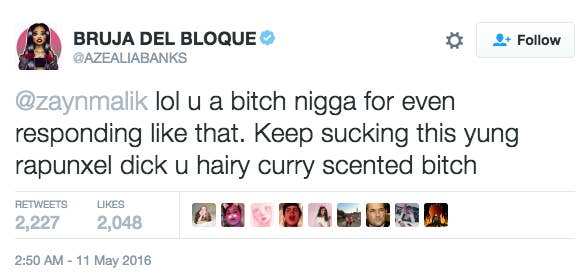
\includegraphics[scale=0.5]{Azealia_banks.jpeg}
  \caption{Azealia Banks tweeting to Zain Malik.}
  \label{fig:azealia_banks}
\end{figure}

Returning now to the first assumption: that neural models can simply rely on input data to identify salient and relevant patterns in the data without human cognition over the relevance of inputs. The strength of neural network models, and in fact machine learning in general, lies in the ability for models to identify patterns in data that correlate to output labels. Thus models construct and manipulate their embodiment of the disembodied data that they are provided. In the construction and manipulation of the model's embodiment of the data lies an implication of the designers' embodiments being reflected in the model. Specifically, through deciding that no higher order representations of the data are to be made, the designers implicitly argue, and embed the normative value that what is relevant to abusive language detection is not human reasoning as to the concept of abuse nor the theoretical and qualitative insights that have been gathered made. Instead, such a practice theorises that there exist some degree of distributed language understanding that renders such cognition irrelevant. Such an (implicit) assumption made by the designers contradicts recent studies that argue that language understanding models do not obtain the ability to understand language, instead they learn to parrot it \citep{Bender-Koller:2020}.

Disregarding for a moment whether such models truly learn to understand or simply parrot language, models that only use surface forms of tokens with the use of pre-trained language models or word embeddings similarly exist on on the globalised end of the model spectrum, albeit further towards the localised end of the spectrum than models that do not use representations optimised on external bodies of data, as these models shift away from the embodiments of the users their data is derived from and further towards the designers' specific positionalities.

\subsection{Model selection}

As a number of models are optimised to identify which model best embodies the data, the designers must make normative decisions to identify what constitutes `best'. In this way, designers reassert their embodiments onto the decision on which model is selected for further use. However, the choice of designating what constitutes `best' is often times a decision that is made prior to any model optimisation. For abusive language detection, best refers to performance for some metrics. For instance, \citet{Gorrell:2018} set out to have a model that has a high precision at the cost of recall. They make this choice to ensure high confidence in their model's predictions of the positive class as their use case is comments made to politicians, where the the ability to criticise without sanction is of particular importance. \citet{Wulczyn:2016} and \citet{Kshirsagar:2018} on the other hand select their models using the Area Under the receiver operating characteristic Curve (AUC) and F1-score, respectively. Both of these metrics for identifying what constitutes `the best performing' model give preference to models that balance classification error, such that models are attuned to false positives as well as false negatives.

Through these choices of metrics we can discern some aims of the modelling process. Where \citet{Gorrell:2018} aim to situate their model within the context of abuse towards British Members of Parliament as it occurs on Twitter, they forego claims of universal applicability. The best performing model, within their understanding is a model which, within the context, produces as few false positives as possible, explicitly accepting that the number of false negatives may be high. Considering then the purpose of their modelling process, it is to allow for embodied downstream analysis of how abuse targets a very specific group. \citet{Wulczyn:2016} and \citet{Kshirsagar:2018} on the other hand develop their models with the aim of obtaining a high degree of generalisation onto the test data in addition to data outside of the sample the model is trained to perform on. Within this goal lies an assumption that there exist an `objective' understanding of what constitutes abuse, which is invariable to the specific embodiments of different users, that is, \citet{Wulczyn:2016} and \citet{Kshirsagar:2018} assume the existence of a global understanding of what abuse is, in addition to an imagined average user that is disembodied from all facets of human life.

\section{Dissertation Models}

Here I consider the two model types that I have developed in \autoref{chap:liwc} and \autoref{chap:mtl}. I document the considerations and assumptions each model type reveals throughout the machine learning pipeline. Rather than go through the entire pipeline, I begin my analysis at the entry points, that the choices of datasets and the modelling choices, as I only make use of previously published datasets.

\subsection{Vocabulary reduction}\label{sub:vocab_redux}

In \autoref{chap:liwc}, I optimised the machine learning models using the datasets published by \citet{Davidson:2017} and \citet{Wulczyn:2016}. The decision to use these datasets as training data stems from the two datasets coming from two distinct sources, Twitter and Wikipedia editor discussions.
To be able to measure the generalisability of the models optimised in \citet{Davidson:2017}, I reduce the multi-class classification task to a binary classification task. Through this reduction in classes, I enforce a normative choice that the detection of abuse has greater value than the identification of the specific type of abuse. Similarly, for all other datasets used for evaluating generalisability (i.e. \citet{Waseem:2016,Waseem-Hovy:2016,Gibert:2018}) are similarly subject to a reduction of output classes, here to align the labels learned by the model with the output labels in these external evaluation sets. My own experiences of hate speech and racialised abuse are at the heart of such a prioritisation.
Further, the modelling choice of how to represent data are also subject to my subjective embodiments. While on one hand the reduction of the input space to a much smaller input space means that the size of the subsequent models, and by extension the complexity of the models.\footnote{I appreciate that even with a reduction of the model size and complexity, neural networks are still too complex to be readily understood without the aid of additional tools.} On the other hand, through such a reduction in the vocabulary, a large majority of words will no longer be represented by the text in the models. Here, my own beliefs that abuse detection models that rely too strongly on the occurrence of specific tokens ultimately provide an issue towards the goal of achieving models that can protect marginalised people from abuse. On the other end of the vocabulary size spectrum, I use byte-pair encoded documents. Due to the nature of generating sub-words, this increases the size of the vocabulary, in comparison to simply using the existing word. I use sub-words and byte-pair encoding to minimise issues of out-of-vocabulary items on the basis of intentional obfuscation of words, e.g. through inserting spaces or punctuation in the middle of words \citep{Rottger:2021}. Moreover, it is motivated by my own lived experiences belonging to a target demographics of abuse and observations I have made of other groups, where people using intentional obfuscation of words, often targets to circumvent simple content filtering techniques, i.e. `moslems' instead of `Muslims'. While the modality I work with is text, such obfuscations also occur in the spoken word through intentional mispronunciation.

In the use of linear models as baseline models, the underlying assumption is that simple correlations of word occurrences with labels, as are found with linear models, do not capture the complex interactions between words in text required to make qualified judgements on abuse. This assumption too is influenced by my own positionality as a brown Muslim who grew up in a predominately white country where brown people, and in particular Muslims, are vilified for their existence. As I am often wont to recount, growing up and watching the news Danish police bulletins for wanted persons frequently used the description `Muslim looking' to describe brown men. Such experiences have made it clear to me that social norms surrounding the use of tokens cannot be readily understood from the words, or multi word expressions without greater contextualisation. For this reason, I use LSTMs as they can capture long interactions between words and are less directly reliant on the occurrence of individual patterns. In addition, a number of past studies having shown the efficacy of CNNs for abuse detection \citep{Park:2017, Mitchell:2019,Kolhatkar:2020,Rizwan:2020,Safaya:2020,Gamback:2017}, I use such models, due to the influence of past work on the topic of hate speech and abuse detection.

As the models described in \autoref{chap:liwc} that only use words or byte-pair encoded words as input rely entirely on the training data to learn patterns in data, its apparent that those models fall towards the very extreme of the globalised end of the spectrum that I propose. On the other hand, while still towards the globalised end of the spectrum, the models that rely on LIWC as the input come are shifted more to the localised end of the spectrum, as the LIWC dictionary that is used to map from words to LIWC categories is informed by considering data external to the data the models rely on.

%{\color{green!80!black}
%\zw{If there is time to add pre-trained embeddings + LIWC embedding layer}
%All models described in \autoref{chap:liwc} fall towards the globalised end of the spectrum, however some further to the extreme ends than others. All linear models that use words or byte-pair encoded data as input represent the extreme globalised-end of the spectrum, as these models only rely on the training data. The linear models that use LIWC categories, and those that use words/BPE in addition to LIWC categories shift slightly towards the localised end of the spectrum by virtue of the LIWC dictionary being developed using external data to inform the creation of the categories.
%As all neural network models use pre-trained word or BPE embeddings, they can be placed further towards the localised end of the spectrum. Similarly to the use of LIWC for linear models, the use of LIWC as additional input shifts the models further towards the localised end of the spectrum.
%}

The motivation for using Byte-Pair encoding is reflected in a) my own personal assumptions about the importance of textual representations and b) computational considerations. Briefly, to minimise the number of out-of-vocabulary items, I use BPE to deconstruct the training data into smaller word-parts, that allow for a) deconstructing words to minimise the influence of intentional obfuscations (e.g. `mooslim women`) of tokens, as I have frequently noted and been subject to abuse that seeks to obscure  and b) better handling of unknown tokens for the computational models.

However, while some models find themselves further towards the localised end of the spectrum than others, all models that I use in \autoref{chap:liwc} are positioned in the globalised end of the spectrum as none of the data representations take into account the local subjective positionality of the individuals in the data, instead they all rely on some abstraction away from the subjective self through processes of disembodiment.

\subsection{Multitask learning}\label{sub:mtl_inchap}

%\zw{If we use current methods}
In \autoref{chap:mtl} I turn to the question of which embodiments, in terms of social constructs such as sarcasm \citep{Oraby_sarcasm:2016}, the basis of a statement \citep{Oraby_factfeel:2015}, and moral foundation \citep{Hoover:2019} in addition to other hate speech and offensive language datasets \citep{Waseem:2016,Waseem-Hovy:2016,Davidson:2017,Wulczyn:2016} would be helpful for a classification model for abuse detection in improving performance on the associated test set.

For this task,  I reuse BPE representations of documents from \autoref{chap:liwc}. therefore some of the embodiments of the models, with regard to text representation remain. Here I focus on those that change for the models described in \autoref{chap:mtl}. Due to the reuse of BPE representations, the analysis of those modelling choices remain the same \autoref{sub:vocab_redux}. However, as I include more datasets into consideration, I also implicitly invite the question `why those datasets'? To answer this question, it's necessary to revisit the aims of each dataset.

One frequently identified issue with computational modelling of abuse is the issue of sarcasm \citep{Rottger:2021} and I use \citet{Oraby_sarcasm:2016}. In this choice lay two assumptions: first, that computational models for abuse detection can benefit from better understanding what constitutes abuse. Second, that there does exist some line between in which sarcasm that mimics abuse is not also abuse. Both assumptions are the result of years of researching online abuse, and in particular exposing myself to the abuse that occurs in online spaces. While I may have become desensitised to abuse through the disproportionate amounts I am exposed to through my research, I frequently see that online abuse, and responses to it, are expressed through humour, in particular sarcasm.\footnote{By responses I mean general reactions and responses to abuse beyond the direct responses to a perpetrator of abuse.}
The second dataset, asks the question of whether an argument is made in the basis of feeling or on the basis of facts \citep{Oraby_factfeel:2015}. As a majority of people who perpetrate online abuse do so infrequently \citep{Waseem-Hovy:2016} an underlying cause for being abusive may well be due to being impassioned, and thus being able to determine whether an argument is made with a basis in feelings or fact may be possible to help improve performance for abuse detection.
We also use a dataset annotated for moral foundation \citep{Hoover:2019}. In this dataset, each document is labelled for which moral foundations it invokes in the annotators. As moral foundations and online abuse can be thought of as concepts that are orthogonal to each other, as moral foundations provide for a higher level of cognition about content that is read, I believe that using such a dataset can aid in optimising a multi-task classifier for the primary task. Here, my own experiences of the harms that occur from being subject to racialised abuse and the apparent desire to inflict such harm from the perpetrators lead me to include this as an auxiliary task.
Finally, I use a number of datasets for online abuse \citep{Garcia:2018,Waseem:2016,Waseem-Hovy:2016,Davidson:2017,Wulczyn:2016}. For this task, I do not reduce the question of detecting to a binary task. However, my subjective positioning does not change from what is detailed in \autoref{sub:vocab_redux}.

Similarly for the choices in developing the data and textual representations, my own subjective embodiments and experiences are a factor in the modelling decisions. This is particularly true for multi-task learning, where I specifically set the weights for how much each task is to contribute to the main task through the frequency of selection. Such a weighting relies on my own consideration of how important each task is to the overall task of identifying abuse. The specific architecture of the model is influenced by their usefulness in prior work \citep{Bingel:2018} and seeking to answer the question of how more complex models would influence the performance on the task.

Using the multi-task learning framework has strong implications for where on the localisation spectrum the models can exist within. For instance, the use multiple different datasets to influence a single model precludes the extreme ends of the modelling spectrum. However, such an optimisation regime also precludes the extremely localised end of the spectrum for the same reason. As each auxiliary task will work, if as nothing else, as a regulariser for the main task. As I use multi-task learning to contextualise the task of abusive language detection within the frame of tasks that have been indicated in prior literature as relevant to the task of abusive language detection, the model is both drawn to a more localised position.
However, as I do not optimise my models on any tasks that seek to make predictions on users, the model does not cross entirely into the space of localised models. Instead the models that I produce, by virtue of learning considerations on tone, argument-basis, sarcasm, and moral sentiment learn some representations of the faculties that I believe of importance to the task. These auxiliary tasks then provide an avenue for the models to be more closely situated within the how each individual person can be represented as a function of how they express themselves. Thus, while further towards being a localised end of the spectrum than the LIWC models, the models fall short of significantly situating the modelling of individuals within the context and lived experiences of that individual.

%{\color{green!80!black}
%\zw{If chapter with Joachim and James is used}
%In \autoref{chap:mtl} I turn to the question of which embodiments, in terms of cultural contexts of the production of abuse matters. Here, I consider the question of whether hate speech that is produced in one cultural context can map to hate speech produced in another cultural context. From this follows then that rather than building a single model or dataset that can be the arbitrator of what constitutes abuse, one can build a model that allows for translations between different cultural contexts. To this end, I explore whether, on the basis of training data alone, a multi-task learning model can learn to bridge two different cultural contexts. Here, I use two different kinds of input with two different expectations and rationales.
% \zw{Text representations: BPE, BoW}
%First, I use a Bag-of-Words (BoW) as input to my multi-task learning model and second, I use BPE encoded data. The use of BPE follows along the logic and reasoning outlined in \autoref{sub:vocab_redux}. The use of BoW as input on the other hand is motivated by the contrast: the wish to represent the data directly. Here the focus is not on obfuscation but on considering the cross-cultural means of expression. For instance the use of the \textit{n-word} with the colloquial `-ga' ending is situated differently in some of the datasets than the same word using the '-er' ending. While both words stem from the same root, they have vastly different meanings and communicate distinct messages \citep{Rahman:2012}. As such, in spite of their shared stem, it can be desirable to retain the two words as distinct tokens as a BoW approach allows for.

% \zw{Dataset choices: Davidson, Waseem \& Hovy, Waseem}
%The motivating factor behind the choice of datasets used is the knowledge that what constitutes hate speech in one cultural context may not constitute it in another. It's therefore necessary to use datasets that represent different cultural contexts, that can then be examined. Rather than using \citet{Wulczyn:2017} in addition to \citet{Davidson:2017}, I use \citet{Waseem:2016,Waseem-Hovy:2016} for two different reasons: The combination of \citet{Waseem:2016,Waseem-Hovy:2016} result in a dataset of comparable size, albeit slightly smaller, than \citet{Davidson:2017}. The second reason for choosing \citet{Waseem:2016,Waseem-Hovy:2016} over \citet{Wulczyn:2017} is that like \citet{Davidson:2017}, \citet{Waseem:2016,Waseem-Hovy:2016} is collected from Twitter, thus allowing one cultural aspect, i.e. the affordances of the platform, fixed while the content and geographic position of the users writing content vary.


% \zw{Globalised-localised model spectrum}
%Using the multi-task learning framework has strong implications for where on the localisation spectrum the models can exist within. For instance, the use multiple different datasets to influence a single model precludes the extreme ends of the modelling spectrum. However, such a training regime also precludes the extremely localised end of the spectrum for the same reason. As each auxiliary task will work, if as nothing else, as a regulariser for the main task.
%As I use multi-task learning to try to learn models that can model abuse across geo-cultural and geo-political contexts, the model shifts in its position on the model spectrum in comparison to single task models. Such a shift happens as some modelling choices draw it towards a more localised model. On the other hand other choices strongly push it towards a more globalised model, the result of which is that only a minor shift happens, in comparison to single-task models using the same data representations. The choices that pull the model towards being more localised is the use of sub-words computed using byte-pair embeddings. As such embeddings are computed outside of the dataset, they provide the data representation, and subsequently the model, with external knowledge on the composition of words. On the other hand, the use of using three datasets for abusive language detection for the main and auxiliary tasks, suggests that any given model will learn some cultural patterns of abuse, but those patterns are limited to two specific instances of abuse, rather than learning about situating the user in their own subjective embodiments. Moreover, as I do not train my models on any tasks that seek to make predictions on users, the model does not cross entirely into the space of localised models.

% \zw{Model choices: MLP}
%Similarly for the choices in developing the data and textual representations, my own subjective embodiments and experiences are a factor in the modelling decisions. This is particularly true for multi-task learning, where I specifically set the weights for how much each task is to contribute to the main task. Such a weighting relies on my own consideration of how important each task is to the overall task of identifying abuse. The specific architecture of the model is influenced by their usefulness in prior work \citep{Bingel:2018} and seeking to answer the question of how more complex models would influence the performance on the task.
%}

\section{Discussion}

Given that subjective choices and biases masquerading as disembodied `objective' positions permeate through the machine learning pipeline, the quest for objectivity and bias-free machine learning becomes redundant. In fact, the search for objectivity in the pipeline creates a veneer of social progress that may cause further harm to already marginalised communities by obscuring and entrenching the dominance of certain bodies over others. Without taking the unique embodiments of all data subjects into account, this imaginary of fair only serves as a justification of maintaining oppressive structures that are inherently harmful and reductive. Considering the question of hate speech detection, developing automated tools that are applied to a general population makes inherent decisions on behalf of the user-group. As such decisions are codified through the machine learning pipeline, they are presented as disembodied and objective decisions on what constitutes hate speech. Through such codification of white perspectives on respectability, attempts to address `bias' only serve to justify existing oppressive structures.

Only by recognising the positionality of the designers of machine learning models can one account for what (and whom) ones own position and the models derived from it privilege and sanction, and the political consequences of these. As data permeates through the machine learning pipeline, a consideration of how data is embodied can empower the designer to answer specific questions that are embodied and mired in context. Such considerations allow designers to interrogate the contexts within which data are created and meaning is made at each step in the dataset creation process. It is through such recognition of context and embodiment that one can realise that as context change, so does the applicability data. 
Further, only by such recognition of the deeply complex nature of embodiment and data can one hope to ask and ascertain which views the models privilege and which are subjugated. For building content moderation systems for hate speech and abuse, the designers of machine learning pipelines can ask how their own embodiments prejudice them to selectively sanction some speech patterns. Moreover, designers may want to ask themselves how such sanctions create downstream implications for the speech that is sanctioned.

Although there are methods with which we can move towards more localized machine learning models, what positions are given space remains a political question.
It is only through wholly representing the context and embodiments of the data creator and the datum that one can hope to arrive at sufficiently localized models. Thus, rather than asking how to eliminate bias and subjective experiences from machine learning in the pursuit of objectivity, shifting the question to consider embodiments would ask us to reflect on the subjective experiences that are given voice. For hate speech detection, such reflections would have designers ask which groups to base their understanding of abuse and the subsequent annotations and models that are derived from it. Such a shift would then require us to ask and reflect upon which bodies' subjective experiences we need to account for to give voice to socially, and computationally, marginalised groups.

%
% \section{Machine Learning as a Conservative Practice}
% \zw{Write about dominant and subjugated discourses for machine learning here; bring in that ML is a conservative practice}
%
% \zw{Citations needed: Foucault on dominant and subjugated discourses, Fraser on subaltern publics, some archival theory on marginalising effects of dominant discourses.i}

